\chapter{Mental Health}

% frame the chapter
Increasingly recognized as a crucial factor for well-being, mental health carries significant economic implications that are often overlooked in favor of more easily quantified conditions, such as physical health. Nevertheless, recent events such as the COVID-19 pandemic shed light on the importance of psychological welfare. 

% economic relevance (social capital, productivity)
Mental health is an economically relevant phenomenon with far-reaching implications that extend beyond individual well-being. Poor mental health often leads to reduced productivity, increased absenteeism, and higher turnover rates in the workplace, directly impacting an organization's bottom line (OECD/EU (2018), OECD/EU (2022)). Furthermore, it places a significant burden on healthcare systems through increased medical costs and utilization of services. The indirect costs, such as loss of income due to disability and the ripple effects on families and communities, further amplify its economic relevance and far outweigh the direct healthcare costs (OECD/EU (2022), WHO (2022)). Therefore, investing in mental health not only enhances individual quality of life but also has the potential for significant economic returns, framing it as a key opportunity in the context of social capital accumulation.

This chapter aims to shed light on the definitions, statistics and dynamics of the topic, with the aim of providing the reader with comprehensive and up to date knowlege in this realm. 

\section{Defining mental health}
% what is MH in general 
    Mental health can be defined as a state of psychological well-being which allows people to cope with demands of life, realize their abilities, learn and work well while contributing to their community. It represents a crucial feature of personal and collective socio-economic develpoment, involving psychological, emotional and social welfare, and affecting how people think, feel and act. 
    Being mentally healthy goes beyond the mere absence of clinically relevant conditions, it encompasses self-esteem, resilience, relationships. Conditions that affect mental health include mental disorders, psychosocial disabilities and mental states associated with impaired functioning, or risk of self-harm. Those affected by these conditions are more likely to report lower mental well-being. 

    % MH risk factors
    Mental health is dynamic and is affected by the interplay of biological factors, environmental conditions and individual experiences. Biological factors such as genetics or substance abuse can create vulnerabilities in all stages of life, but events that occur during developmentally sensitive periods are particularly impactful. Harsh childhood experiences in the form of bullying, physical and psychological abuse and poor health can have long lasting negative consequences on an individuals' mental condition. On the other hand, mental resilience can be promoted through building social and emotional skills, providing youths with positive interactions, safety and community as well as quality education. 
    Thus, mental health can be though of as a continuum ranging from an optimal state of well being, to debilitating states of great suffering and emotional pain (WHO, 2022).

    When dealing with circumstance that can exacerbate mental ill-health, a distinction can be made between local factors which affect individuals, families and communities on a small scale, and global or systemic factors which generate vulnerabilities for the entire population. Among the latter we find key threats such as economic crises, disease outbreaks, humanitarian emergencies, displacement and climate crisis related events, as well as sociocultural and geopolitical factors such as infrastructure, inequality, social stability and environmental quality. 
    
    % MH protective factors
    Although exposure to risk factors undermines mental health, most at-risk people will not develop conditions, while many without known risk factors will develop them. In this perspective, encouraging protective factors strenghtens resilience in the population. On the individual plane, building strong social and emotional skills, a solid sense of self-worth and healthy habits such as keeping physically active are key in generating resilient individuals. Other individual protective factors include a nurturing and supportive family environment from a very young age, decent working conditions and a cohesive social network. On the structural level, protective factors manifest in economic security, easy and equal access to services, social protection, qualitable infrastructure and economic security, as well as social integration and contained inequality.  


        



\section{Global epidemiological overview}
    % define relevant MH issues --> depression, anxiety, suicide stats
    Mental health conditions are prevalent in the population, with about one in eight people worldwide living with a mental disorder (WHO, 2022). Heterogeneity in their distribution emerges according to age, gender and other individual characteristics. Overall, disorders related to anxiety and depression are the most common, and suicide accounts for more than one out of one hundred deaths (WHO, 2022). 
    % seeking help
    Still, seeking help for mental health conditions is hindered by low mental health literacy, poor service quality, cost of care, stigma and discrimination, making for underdiagnosis of all conditions. 

    % service provision not commisurated with needs
    Worldwide, mental health conditions are severely underserviced due to lack of information and research, as well as deficient provision of resources and services. On average, less than 2\% of health care budgets are dedicated to mental health, and out of that more than 70\% of mental health expenditure in middle-income countries is dedicated to psychiatric hospitals (WHO, 2022). 
    Furthermore, professionals such as psychiatrists and psychologists are scarce relative to the population, and gaps in service coverage are amplified by quality and cost of care across countries. 
    % measurement challenges
    Additionally, measurement of mental health condition is hampered by incomplete data, outdated information and cross-cultural differences in the conceptualization and tracking of conditions. 

    % quick stats


    % this section
    This section seeks to offer current statistics on the global prevalence and diversity of mental health conditions, with a particular emphasis on the OECD region prior to the COVID-19 pandemic. Before delving into a data-driven discussion on this subject, it is essential to first clearly define the two most pertinent categories of mental disorders under consideration: anxiety and depressive disorders. 


        % anxiety       [  %  TO DO  %  ]
        \subsection{Anxiety disorders}
        \begin{figure}  % anxiety OECD rates figure
            \centering
            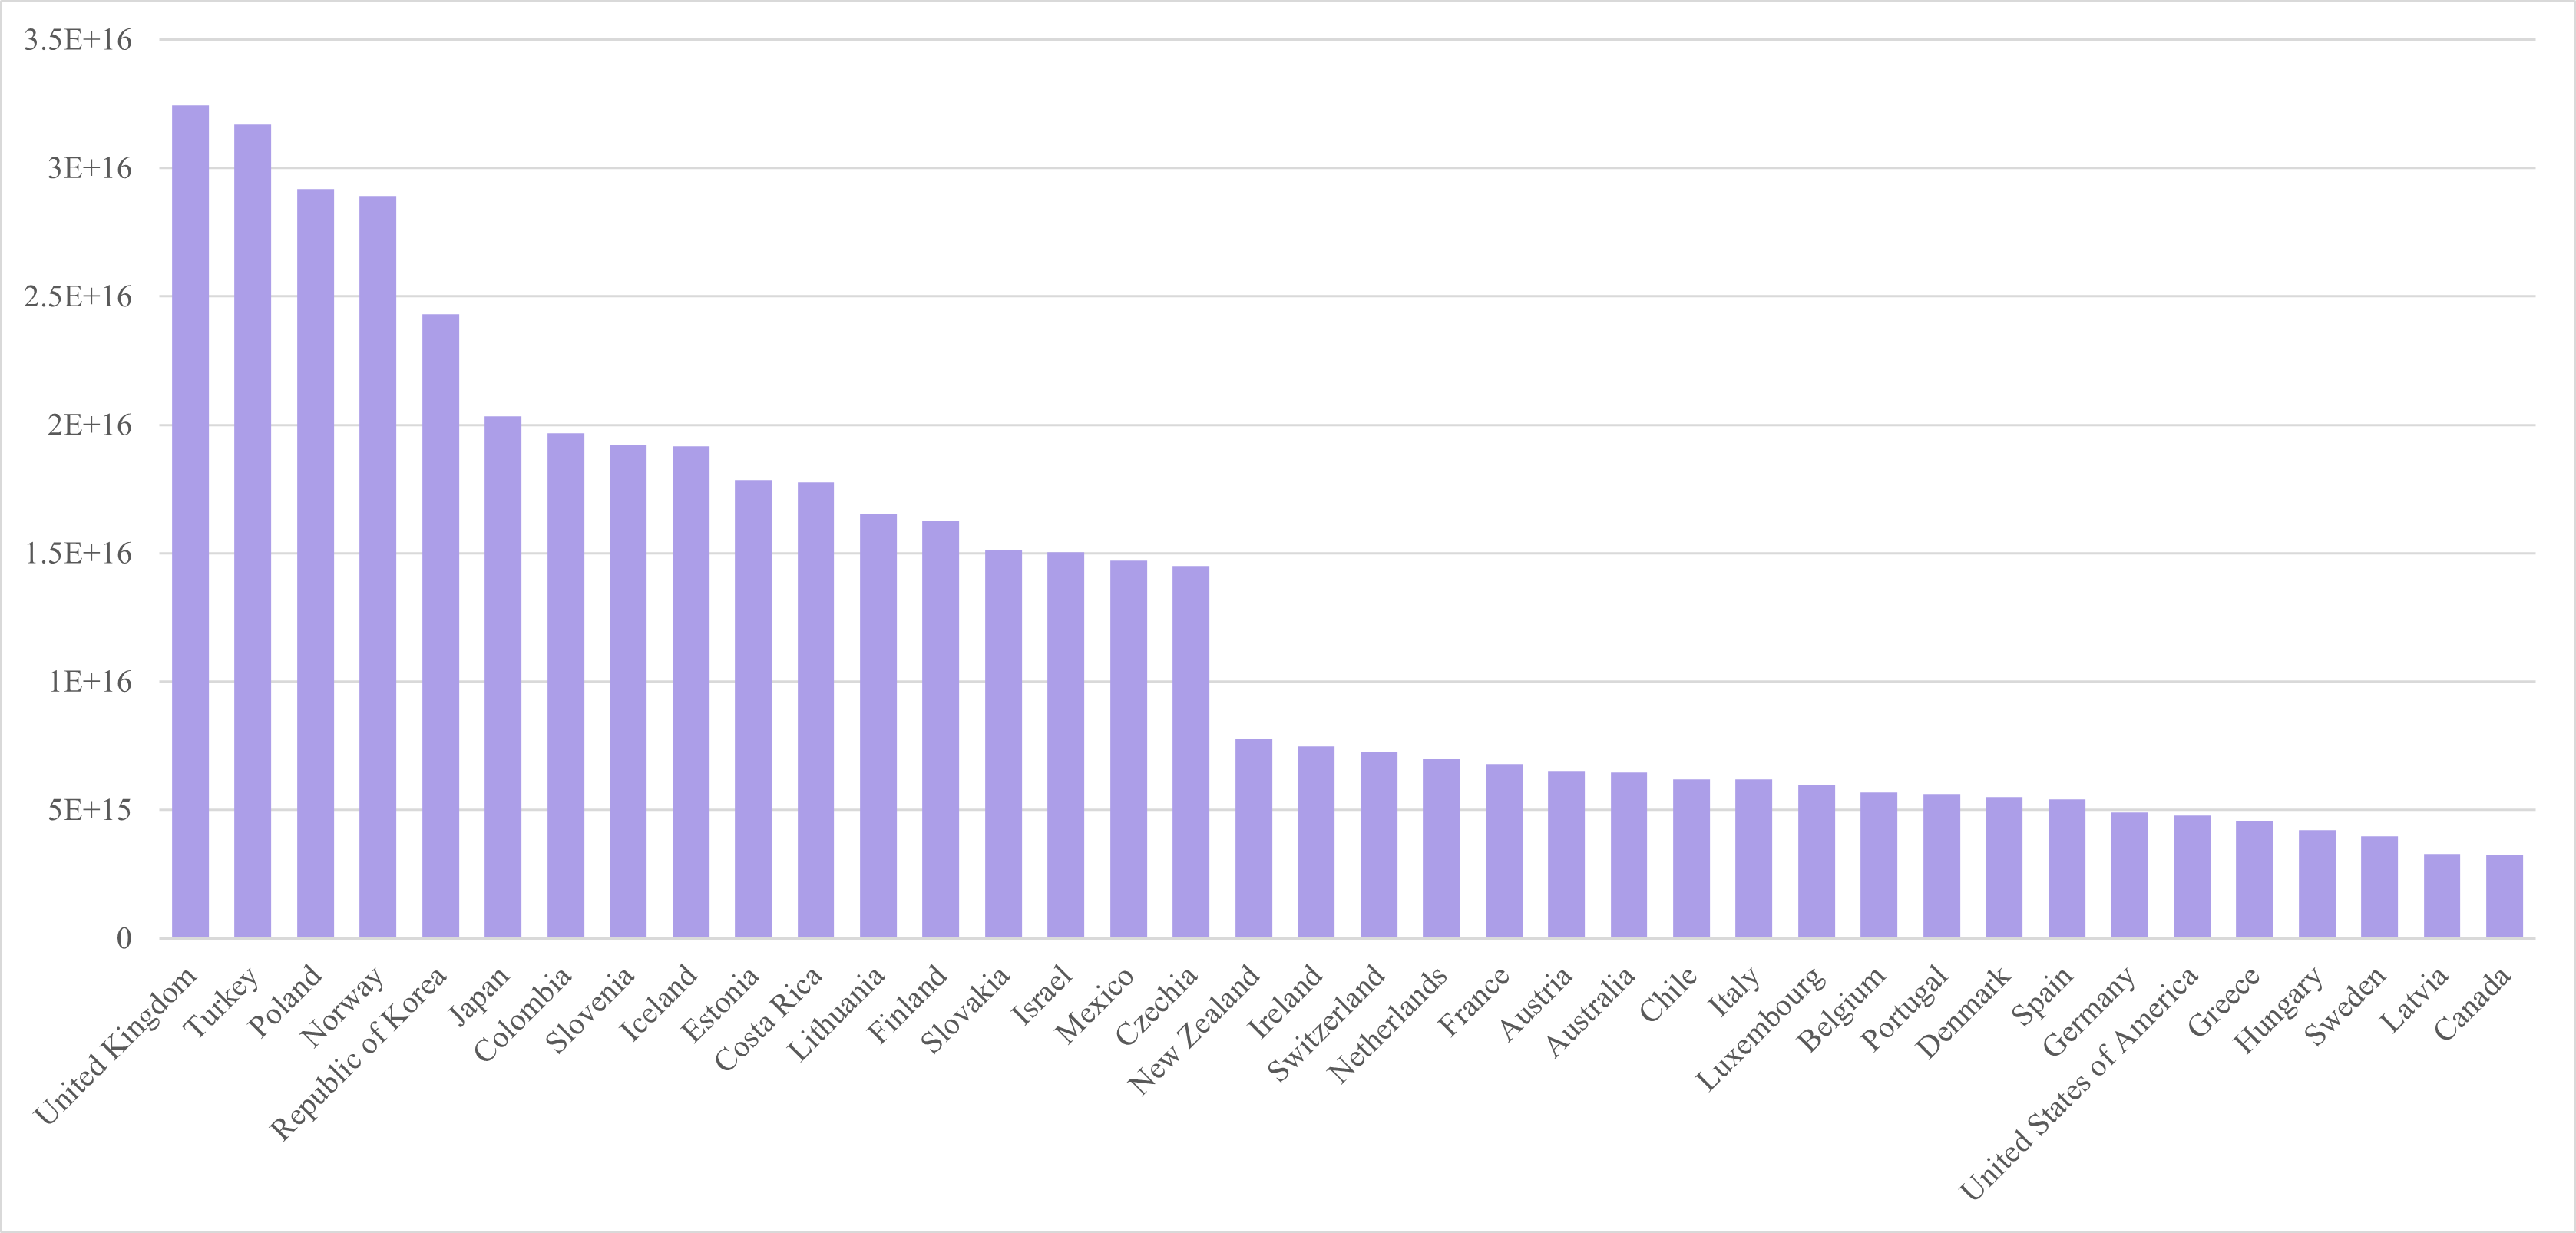
\includegraphics[width=\textwidth]{GRAPHS/1MH_anxietydisordersOECDprevalence100k2019.png}
            \caption{\emph{Prevalence of anxiety disorders per $100 000$ inhabitants, 2019.
            Source: GBD (2019).}}
            \label{fig:anxiety_OECD}
        \end{figure}

        % depression    [  %  TO DO  %  ]
        \subsection{Depressive disorders}

        \begin{figure}  % depression OECD rates figure
            \centering
            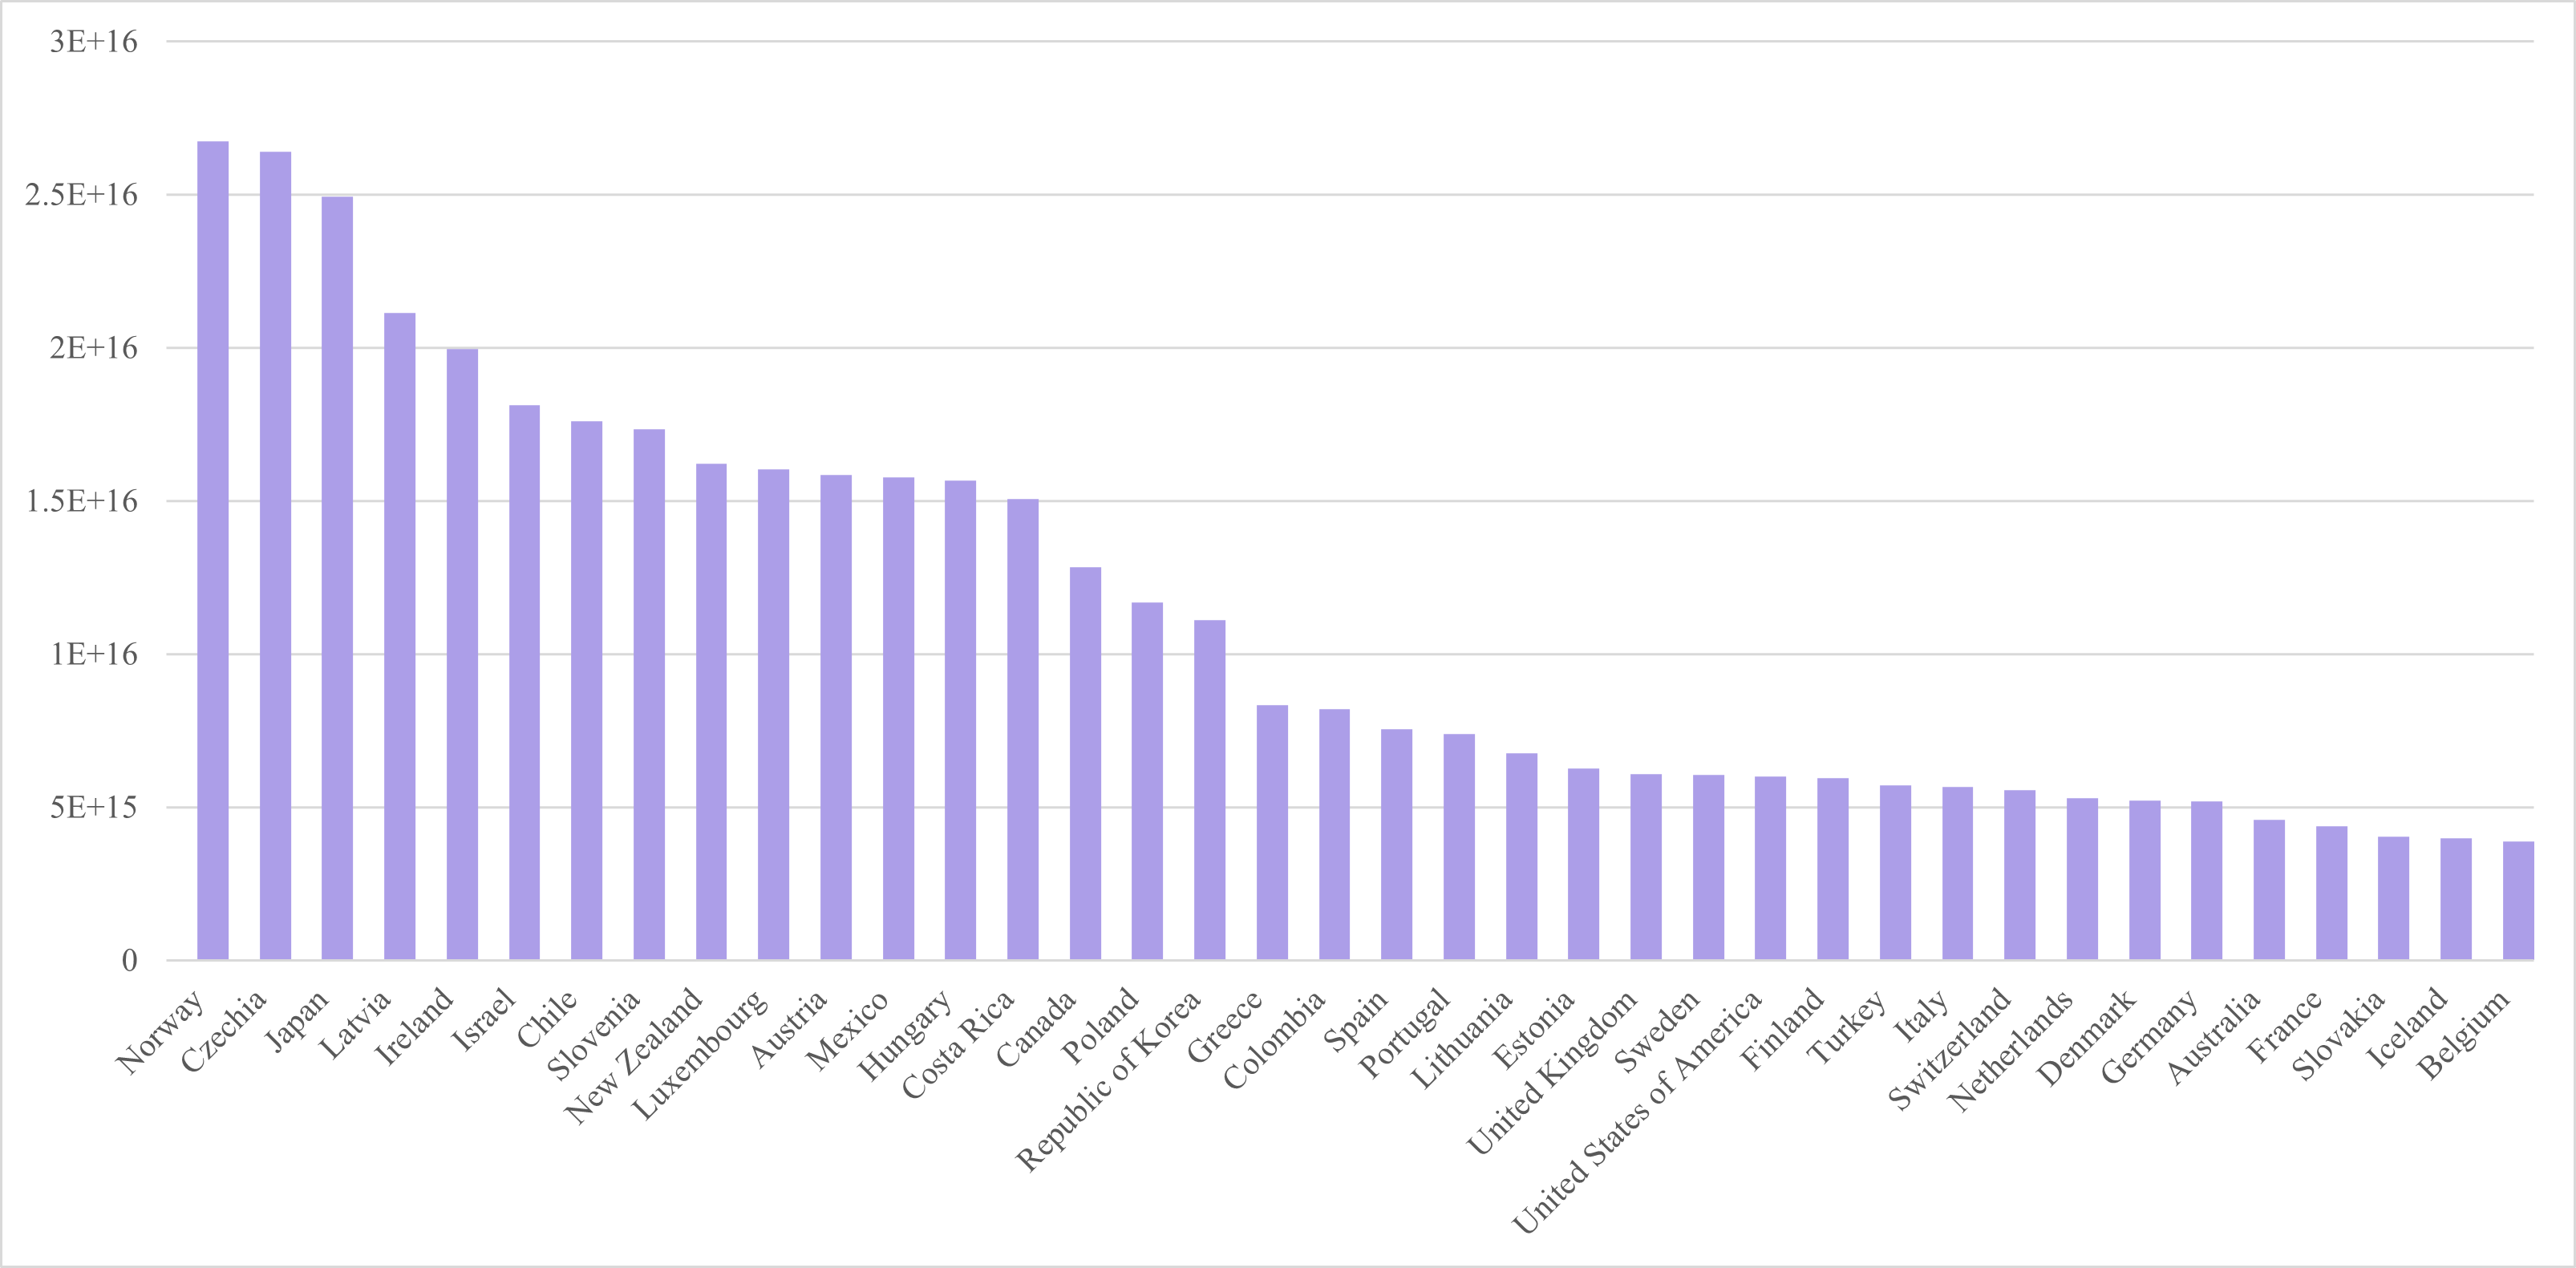
\includegraphics[width=\textwidth]{GRAPHS/1MH_depressivedisordersOECDprevalence100k2019.png}
            \caption{\emph{Prevalence of depressive disorders per $100 000$ inhabitants, 2019. 
            Source: GBD (2019).}}
            \label{fig:depression_OECD}
        \end{figure}




    


\subsection{Heterogeneity determinants}

% statistics using WHO and EUROSTAT data references
    % risk factors and general trends
\paragraph{Gender differences}

\paragraph{Cohort specificity}

\section{Measurement via psychometric tools}
% how is it measured




\section{COVID-19's mental burden}
    The COVID-19 pandemic has had a profound impact on mental health, manifesting in distinct but interconnected local and global threats. At the local level, individuals have reported higher rates of anxiety, depression and stress related symptoms, driven by social isolation, disruption to daily activities and heightened uncertainty. On a broader, structural scale, the pandemic has significantly compromised healthcare delivery, a disruption of particular impact for those with pre-existing mental health conditions. Overall, this has had a disproportionate impact on vulnerable and disadvantaged populations, further widening existing inequalities. 
    Public health emergencies of this kind can be platforms for change, driving improvement of public services and structural investments in the name of public interest, focused on education, prevention and effective treatment aimed at rehabilitation. 

    %   stressors
    The pandemic increased the prevalence and intensity of mental health stressors. The most immediately evident one is fear of the health effects of the virus, a concern that was particularly acute during the periods of maximum uncertainty surrounding its nature and transmission. Contracting the virus introduces an additional layer of adversity, encompassing not just the physical symptoms, but also the psychological toll linked to the illness and its potential long-term effects. Additionally, the emotional burden of bereavement adds yet another dimension to the mental health landscape.
    Public health containment measures, such as distancing and quarantining, imposed social isolation and loneliness on many, generating feelings of helplessness and putting strain on the individual's relationships. Loss of routine and abrupt change to daily activities has negatively impacted the youth and the older component of the populations. 

    %   work
    COVID-19 exacerbated uncertainty for the work force, causing spikes in unemployment and plunging many into financial adversity. Both unemployment and poverty are known risk factors for mental health conditions, and gloabl projections for extreme poverty have been revised upwards (Lakner et al., 2020). 

    % service disruption
    Furthermore, as COVID-19 spread, almost all mental health services were disrupted or suspended. Almost 

    %   negative coping
    Negative coping mechanisms for psychological distress and symptoms of anxiety and depression may include resorting to alcohol, drugs and other addictive behavior, including but not limited to technology aided gambling, gaming and excessive use of social media. 


